\documentclass[12pt,a4paper]{article}
\usepackage{fontspec, xunicode, xltxtra}
\usepackage{cite}
\usepackage{caption}

\title{基于攻击图的组织网络安全风险分析技术研究进展\\Survey of Attack Graph Based Organization Network Security Risk Analysis}
\author{软件与微电子学院\\胡天翔\\1501110661}
\setmainfont{STFangsong}
\XeTeXlinebreaklocale "zh"
\XeTeXlinebreakskip = 0pt plus 1pt
\begin{document}

\maketitle

\renewcommand{\figurename}{图}
\renewcommand{\abstractname}{摘要} 
\begin{abstract}
\setlength{\parindent}{0pt} \setlength{\parskip}{1.5ex plus 0.5ex minus 0.2ex} %\noindent
为了解决在计算机网络,特别是组织网络中存在的多阶段、多步骤攻击的防御问题,一项针对网络、脆弱性和攻击者模型进行静态分析的技术——攻击图(Attack Graph)被提出,其通过对整个组织网络进行探测,确定网络的拓扑架构,分析资产存在的脆弱性,并且利用公共漏洞信息库和攻击模式库这些信息进行建模,最后利用图论、博弈论等方向上的算法,对模型进行分析,从而使得我们能有能力回答这样一个问题:“我们的网络到底有多安全?”
\paragraph{关键字}计算机网络;系统安全;攻击图;安全度量;网络加固
\end{abstract}

\section{简介}

\paragraph{}
目前,计算机网络已然构成了诸多信息技术基础设施的核心组成部分,这些设施包括电网、金融数据系统和应急通信系统领域等。保护这些网络免受恶意入侵对国家的经济和安全至关重要。我们常常能够在被利用来攻击这些系统的软件/应用中发现脆弱性,而攻击者就是利用这些被公布或者没有被公布的脆弱性方才得以实施攻击。
\paragraph{}
但是就目前而言,组织网络的安全风险管理与其说是科学,不如说是一门艺术。系统管理员通过直觉和丰富的经验来操作,而不是依靠客观指标来指导和证明决策的制订。
\paragraph{}
攻击图技术旨在用于解决此类场景的问题,其包括可用于客观的模型和指标,评估企业网络中的安全风险的分析技术,以及指导管理员使用模型和指标帮助进行网络防御决策的理论和方法。
\paragraph{}
为了提高组织网络的安全性,有必要测量由不同网络配置提供的安全性。攻击图研究的目的是开发一个标准模型,用于测量计算机网络的安全性。标准模型将使我们能够回答诸如“我们比昨天更安全吗?”或“一个网络配置的安全性如何与另一个进行比较?”这样的问题。另外,有一个标准模型来衡量网络安全可以使用户,软件供应商和研究人员能够一起评估网络安全的方法和产品。
\paragraph{}
对于组织网络的安全风险分析主要有如下挑战:
\subparagraph{安全漏洞非常泛滥}
CERT\cite{2}每周会报告约100个新的安全漏洞,这使得对于企业网络的安全管理(包括数百主机、每个主机上不同操作系统和应用程序以及它们上存在的可被利用的漏洞)非常困难。
\subparagraph{攻击者发起的多步骤攻击}
相比以前攻击者仅能发起简单的原子攻击而言,现在的攻击者为了能够突破各类防火墙/网关的防御,往往会采用多步骤、多宿主的攻击,逐渐渗透进整个网络,最终危及到关键系统。但是其每一步骤却又不足以引起防护系统的警报,这使得对于关键系统的保护具有挑战性。
\subparagraph{现有防御手段不能处理攻击的复杂性}计算机系统遭受的攻击逐渐增多,当一个新的漏洞被报告出来后,攻击者可以非常快速的开始使用这个漏洞。传统的攻击检测方式(如入侵检测系统IDS)具有太多诸如误报、低可拓展性和检测攻击的限制方面的问题。
\paragraph{}
良好的评价指标应当具有如下性质:其是一致的、收集成本低、数字表示、有度量单位和具体的上下文\cite{2}。 攻击图技术通过捕获漏洞之间的相关性,并以实际攻击者渗透网络的方式来测量安全性,从而应对这一挑战。通过网络分析所有攻击路径,提供整体系统的风险指标。通过这个指标,可以分析安全成本和安全利益之间的权衡。因此,决策者可以避免过度投资无法产生实际效果的安全措施,或避免投资和风险造成毁灭性后果。攻击图技术的度量是一致、明确的,并为理解计算机网络的安全风险提供了上下文。
\paragraph{}
本篇综述将以如下形式组织:第2章展示近年来攻击图本身元模型以及对应的生成算法方向的研究。第3章则介绍攻击图分析算法方向的研究。第4章介绍在安全分析中所面临的一些挑战。最后在第5章给出总结。

\section{攻击图及其生成技术}

\paragraph{}
攻击图对如何将多个漏洞组合起来进行攻击这一问题进行建模。它们使用一系列安全相关的条件来表示系统的状态,这些条件包括特定主机上特定漏洞的存在、不同主机之间的连接关系等。对脆弱性的利用则被建模成为状态之间的转移。

\paragraph{}
例如,在图1当中,左侧展示了一个典型的网络配置,右侧则展示了恶意工作站用户对数据库服务器造成损害的攻击图。 在网络配置中,防火墙旨在帮助保护内部网络。内部文件服务器提供文件传输(ftp),安全shell(ssh)和远程shell(rsh)服务。内部数据库服务器提供ftp和rsh服务。防火墙允许从用户工作站到这两个服务器的ftp、ssh和rsh流量,并阻止所有其他流量。
\begin{figure}[!htp]
	\centering
	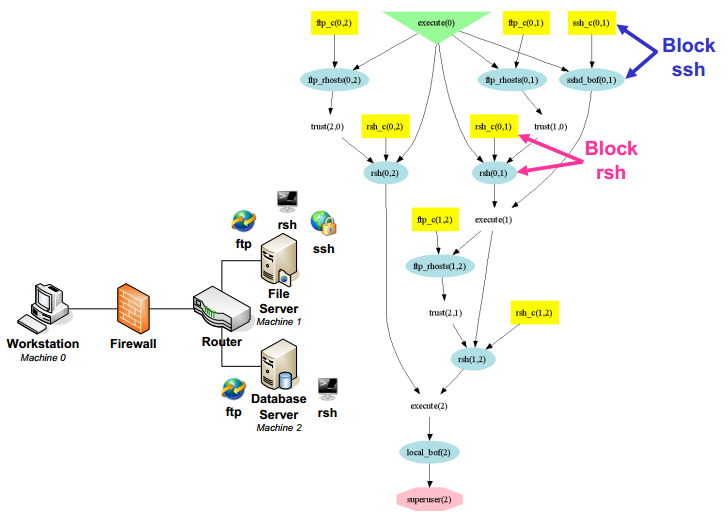
\includegraphics[scale=0.5]{images/example.png} 
	\caption{样例网络配置及其对应的攻击图}
\end{figure}

\paragraph{}
图中描述的攻击图包含如下三条攻击路径:
\subparagraph{1}$sshd\_bof(0,1)\rightarrow ftp\_rhosts(1,2)\rightarrow rsh(1,2)\rightarrow local\_bof(2)$
\subparagraph{2}$ftp\_rhosts(0,1)\rightarrow rsh(0,1)\rightarrow ftp\_rhosts(1,2)\rightarrow rsh(1,2)\rightarrow local\_bof(2)$
\subparagraph{3}$ftp\_rhosts(0,2)\rightarrow rsh(0,2)\rightarrow local\_bof(2)$

\paragraph{}
第一条攻击路径从结点$sshd\_bof(0,1)$开始,这个结点表示了一次从主机0(也就是工作站)向主机1(文件服务器)发起的缓存区溢出攻击(向ssh服务发起的)。在一次缓存区溢出攻击当中,一个程序的某个变量被编写成只能够存储固定长度的数据,但是一旦向其提供超出这个长度的数据,就会将多余的数据顺序写入相邻的内存区域当中,从而使得攻击者能够在文件服务器上执行任意的代码。$sshd\_bof(0,1)$的后继节点$ftp\_rhosts(1,2)$从而就可以开始执行,其表示的攻击为攻击者利用特定的ftp漏洞,将一个可信主机列表从主机1(文件服务器)上传给主机2(数据库服务器),从而使得攻击者可以将他自己电脑远程ssh到数据库服务器,而不需要提供密码。但此时攻击者在主机2(数据库服务器)上还只拥有一般的用户权限,所以接下来的$local\_bof(2)$,表示攻击者利用本地具有root权限的服务的缓存区溢出漏洞发起攻击,来获取完整的控制权限。

\subsection{攻击图生成方法研究}
这部分主要介绍目前存在的一些攻击图生成方法及已经存在的工具。
\paragraph{1)State Enumeration Based Approach(基于状态枚举的方法)}
这种攻击图生成方法是所有生成方法最为原始的,其使用的攻击图元模型被称为State Enumeration Graph,即状态枚举图。图中的每个结点表示所有主机、服务和攻击者的一个状态集合,结点之间的连边表示攻击者在特定状态下可以发起一次原子攻击以及这次攻击攻击会产生的后果,从而使得结点能够通过这样的边到达新的结点。另外也有将图结构推延模型和对图所期望性质的模型建立出来,然后将生成分析工作交给模型检查工具方向的研究,但是其本质上都是对状态空间的一个枚举。这类生成方法最后生成出的攻击图的大小规模相对组织网络规模在指数级,难以应用在实际场景当中。
\paragraph{2)TVA(网络脆弱性的拓扑分析方法)}
在文献\cite{3}\cite{4}\cite{5}当中,作者描述了一种用于生成攻击图的工具。这种方法提出了关于攻击的单调性假设,即“攻击者可发起原子攻击的集合不会因为新原子攻击的加入而减少”,虽然这个结论在现实生活中不一定往往存在(例如缓冲区溢出可能导致服务器的宕机,从而使得攻击者无法进行之后的攻击操作),但是它成功的将原本状态枚举方法中指数级的攻击图规模缩小到了多项式级别。它的核心理念在于使用利用依赖攻击图(Exploit Dependency Graph)来表示攻击的前置条件和后置条件,在分析过程中,可以使用当前已经可以访问到的全部攻击结点的集合来应对状态枚举方法中的单个状态结点。基于这种方法,我们可以通过图搜索算法来链接独立的脆弱性并且寻找可能的攻击路径集合。
\paragraph{}基于这类生成方法和元模型架构的网络安全分析工具Cauldron现已正式商业化,并且在美国许多关键政府部分中得以应用。
\begin{figure}[!htp]
	\centering
	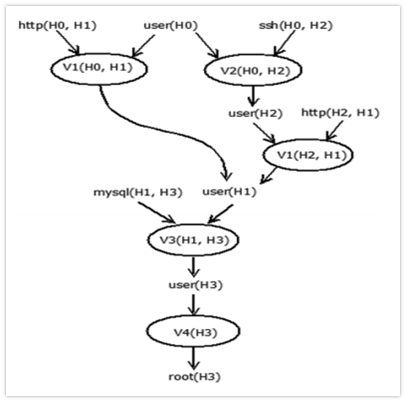
\includegraphics[scale=0.7]{images/TVA.png} 
	\caption{基于TVA方法生成的攻击图}
\end{figure}
\paragraph{}
图2表示了基于TVA方法生成的一个样例攻击图:
\paragraph{3)NetSPA(网络安全计划架构)}
在文献\cite{6}\cite{7}中,作者使用攻击图来模拟对手和简单反制措施的效果。 它使用防火墙规则和网络漏洞扫描工具创建组织网络的模型。 然后,它使用该模型来计算网络可达性和多先决条件攻击图(Multiple-Prerequisite Attack Graph),以表示对手利用已知的漏洞发起攻击的潜在路径。这会发现所有攻击者从一个或多个位置开始并最终能够入侵的主机。NetSPA生成的攻击图规模通常随着典型网络中主机数量的增加而缩放为$O(nlogn)$。而通过测量攻击者可以攻陷的总资产(数量、价值),可以评估不同攻击者的风险。
\begin{figure}[!htp]
	\centering
	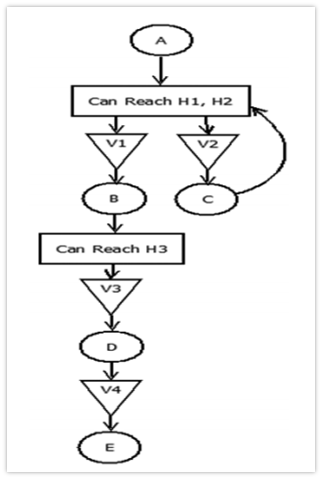
\includegraphics[scale=0.7]{images/NetSPA.png} 
	\caption{基于NetSPA方法生成的攻击图}
\end{figure}
\paragraph{}
图3表示了基于NetSPA方法生成的一个样例攻击图:
\paragraph{4)MulVAL(多主机、多阶段的脆弱性分析)}
文献\cite{8}\cite{9}中,作者描述了一种基于Datalog的网络安全分析器。脆弱性数据库中的信息、每台主机的配置信息和其它的一些相关信息都通过程序的加工处理编码成为Datalog中的事实,从而供推理引擎分析,计算出网络中各种组件之间的交互。MulVAL最后生成的逻辑攻击图(Logical Attack Graph)的规模随着网络规模大小的变化为$O(n^2)$。
\begin{figure}[!htp]
	\centering
	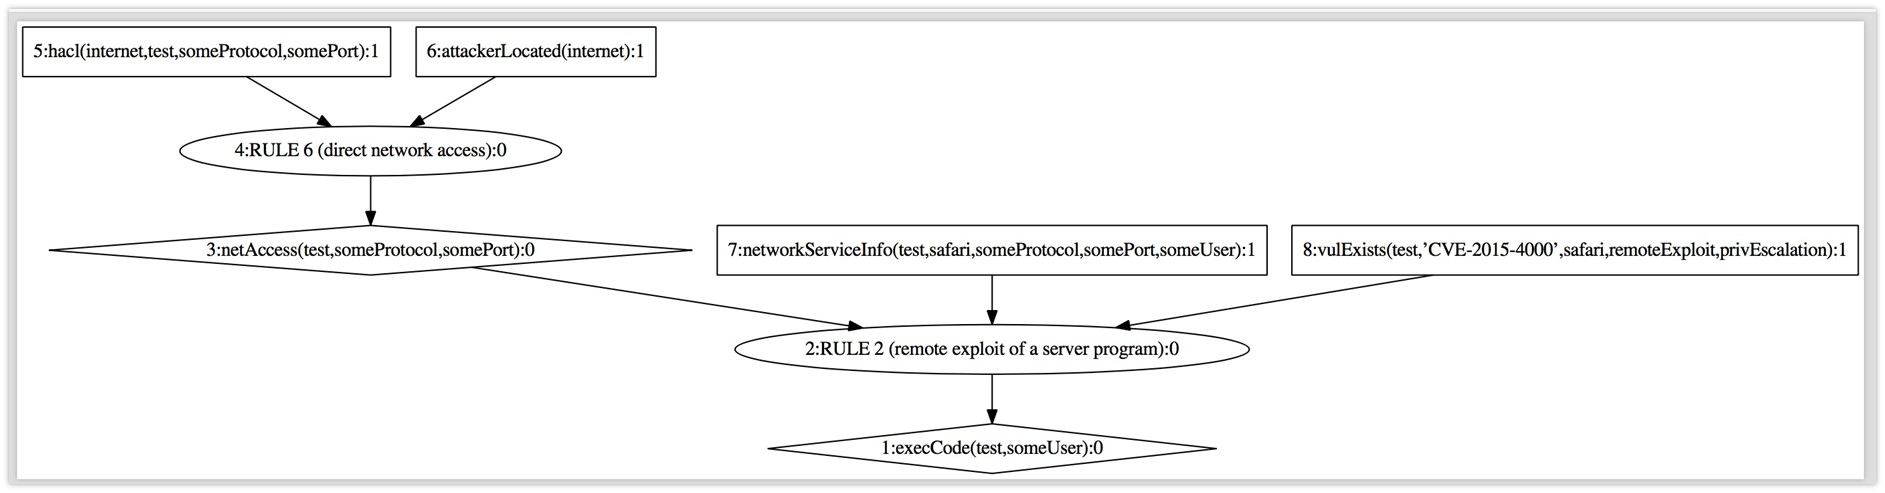
\includegraphics[scale=0.40]{images/MulVAL.jpg} 
	\caption{基于MulVAL方法生成的攻击图}
\end{figure}
\paragraph{}
图4表示了基于MulVAL方法生成的一个样例攻击图:
\paragraph{}
MulVAL本身作为一个开源项目被公布给世界范围内的研究者和组织进行使用,是目前攻击图领域知名度最高的攻击图生成工具。

\paragraph{}
文献\cite{10}\cite{11}\cite{12}\cite{13}中,描述了一些最近用于进行脆弱性分析和攻击图生成的工具。Skybox Security\cite{10}和Red Real Systems\cite{11}已经开发出了一款可以用于生成攻击图的工具。
整个系统的风险是通过每条路径的成功概率乘上对应攻击目标受损的损失之后求和而进行计算的。Nessus\cite{12}和Retina\cite{13}则是脆弱性管理工具,可以帮助组织对脆弱性进行评估、迭代和保护。

\subsection{攻击图生成效率研究}
\paragraph{}
除开基于状态枚举的攻击图生成方法来说,其它三种攻击图生成方法从效率和能力上来说的差距其实是不大的,事实上,在近年的攻击图研究发展中,有关攻击图生成方向的研究不再主要以尝试发明新的攻击图元模型,而是更多的集中于研究如何提高攻击图的生成效率。

\paragraph{}
最近两年的两篇文献\cite{14}\cite{15}均提出了在构建攻击图的过程中,利用并行化解决攻击图规模巨大的一种思路。在构建攻击图的过程中,随着机器、服务以及其上的漏洞等元素数量的增加,攻击图的规模也逐步增加,而对攻击图的计算(NP-Hard)也会随之增加,从而使得对于大规模网络的计算非常困难。所以,对于攻击图构建的并行算法就变的很重要。所以这篇文章提出了一种基于分布式内存的并行算法,用来在分布式的代理平台上搭建攻击图的分布式计算。为了实现这个算法,要求对平台所使用的内存进行抽象,成为一个虚拟的、共享的内存,并通过分割网络互相可达的信息来对内存进行初始化。随后文章对这个算法进行了评估,发现即使是较小程度的并行,在生成算法复杂度较高的情况下也会为计算性能带来非常大的提升。

\section{攻击图分析技术研究}
\paragraph{}
攻击图元模型和攻击图生成技术其实都仅仅是将组织网络、脆弱性、攻击模式等安全相关信息使用建模的方式进行表示,并且关联了起来。虽然更加直观的展示组织网络中存在的各类信息以及他们的之间的关系,但是么有提供任何评估、分析方面的内容,而这就是攻击图分析技术研究所进行的工作。

\paragraph{}
对于攻击图的分析主要有如下一些:

\subsection{安全度量指标}
\paragraph{}
对于一个组织网络来说, 其最主要的分析工作就是各项安全指标的度量,这项工作使得我们能够回答“今天的网络是否比昨天更加安全?”这样一个问题。
\paragraph{}
基于攻击图的度量标准十分复杂多样,目前并没有一个完全的、可信的度量标准,同时许多直观上感觉较为可信的度量标准也经常容易被人们不断推翻。但总的来说,具有代表性的标准有这样一些:
\subparagraph{Network compromise percentage\cite{27}}网络中有多少主机可以被攻击者获取用户或管理员权限(考虑资产价值)
\subparagraph{Weakest adversary security metric\cite{28}}最弱对手:攻击者至少需要多少前置条件才可以完成攻击
\subparagraph{Shortest path metric / number of paths metric / and mean of path lengths metric\cite{29}} 最短攻击路径 / 攻击路径数量 / 攻击路径平均长度

\paragraph{}
Cauldron的作者Noel S.和Jajodia S.在2014年一篇文献中对攻击图度量的指标进行了分簇,如下图5所示:
\begin{figure}[!htp]
	\centering
	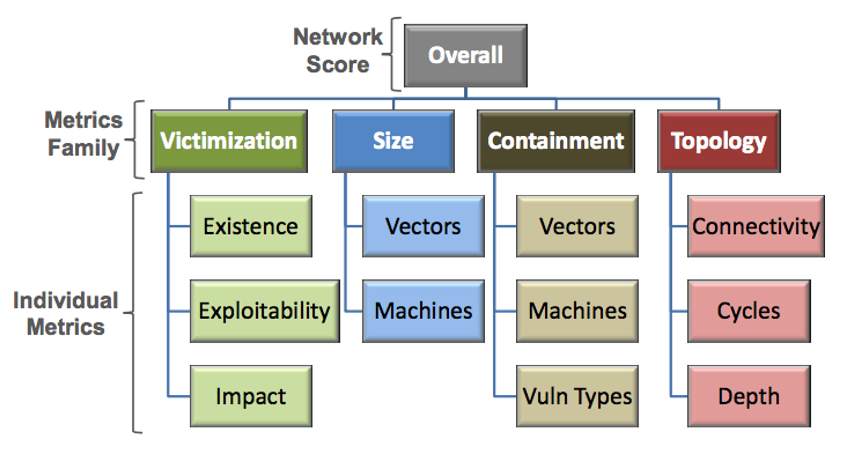
\includegraphics[scale=0.40]{images/metrics.png} 
	\caption{攻击图度量指标簇}
\end{figure}

\paragraph{}
基于这样的一些安全度量指标,我们就能够对整个组织网络的安全态势,给出基本的判断——“一个网络到底有多安全?”

\subsubsection{攻击面分析}

\paragraph{}
除开单纯数值上的分析,我们还可以对图结构进行更多的分析,其中最为主要的就是攻击面分析。攻击面分析的本质在于求解所有攻击路径,直观展示攻击者可以采用的攻击路线,便于后续对这些攻击路线的深层分析。

\paragraph{}
路径的深层分析一方面包括路径代价分析,即首先确定每条路径的长度(或者说原子攻击的数量),然后就可以结合原子攻击的代价/成功率信息,计算整条攻击路径的代价/成功率。另一方面则是对结点进行分析,包括“关键结点”的计算,即一定存在于攻击路径上的点,修复任何一个关键结点则所有的攻击路径失效。由于关键结点并不一定存在,所以可以进一步对结点权值进行计算,通过途径此结点所有攻击路径的代价、成功率以及目标价值,计算这个结点的收益权值,提供给决策者进行修复决策。

\paragraph{}
图6为一个典型的路径分析结果展示:
\begin{figure}[!htp]
	\centering
	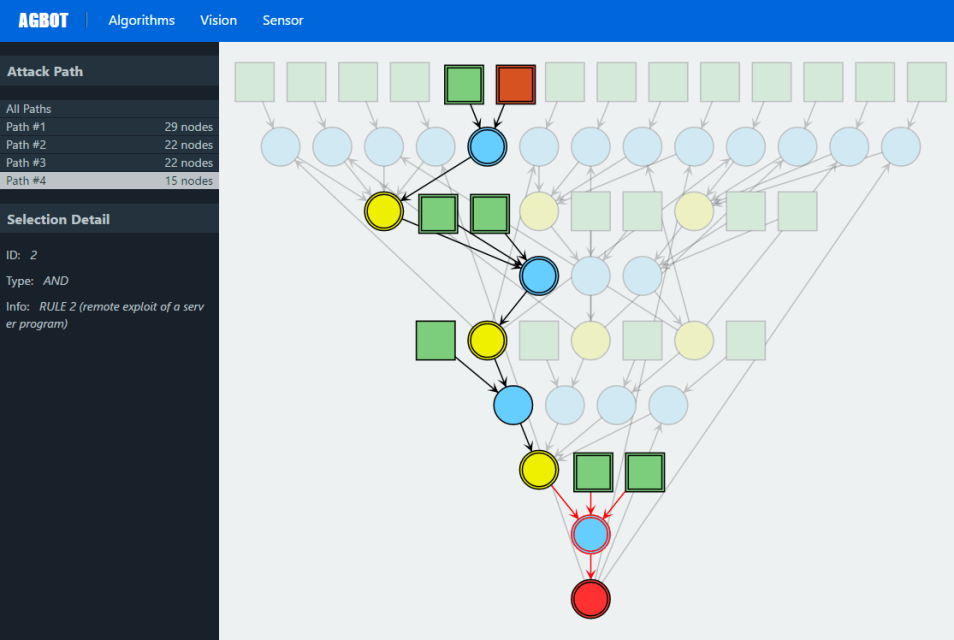
\includegraphics[scale=0.40]{images/paths.png} 
	\caption{基于工具AGBOT生成的攻击路径可视化}
\end{figure}


\subsection{防御措施研究}

\paragraph{}
在攻击图生成后,防御者可以采用许多方式来进行防御,攻击面分析会对整个组织网络中容易遭受攻击的结点、重要的结点、性价比最高的结点进行列举,系统管理员可以根据这些信息进行相关的修补工作,从而提高整个系统的安全性能。

\subsubsection{Attack Graph Games}
防御者进行修复之后并不是话题的结束,攻击者同样可以针对这些防御手段进一步强化攻击,所以就形成了一种博弈问题。
\paragraph{}
从14年至今,Czech Technical University的Karel Durkota带领的研究小组对攻击图博弈问题(Attack Graph Games)进行了许多研究\cite{18}\cite{19}\cite{20}\cite{21}\cite{22}\cite{23}。以\cite{19}为例,这篇文章主要是提出了利用攻击图对网络和攻击者建模之后,利用博弈论算法计算可能的攻击路径以及相应的解决方案的一种思路。他的整体解决方案,是对Stackelberg security games的拓展,外加两点定制:1)对攻击计算机网络的策略使用攻击图来进行建模;2)防御者使用骗局(蜜罐)而非直接分配资源来加固网络,即网络管理员(防御方)主要采用的手段是在系统中设置蜜罐,蜜罐不会同合法用户进行交互,而是引诱和干扰攻击者,并向管理员报告攻击警报、收集攻击者的详细信息。但是蜜罐的设置和维护的消耗非常大,决定在什么地方设置、如何设置是困难的。同时有情报来源的攻击者也会充分了解这些信息,从而尝试规避它们。
\paragraph{}
这篇文章认为虽然直接对广义的攻击图进行计算是NP-Hard的,但是从安全加固的角度来看,其对攻击者的动机和可能的行动顺序等信息的提供是非常有帮助的。所以文章提出了一种将攻击图转变为MDP,并且引入一系列的剪枝技巧来降低计算复杂度的解决方案;并且提出了对模型和解决算法基于经验的验证,并对可拓展性进行了验证,对现实情况进行求解的类型以及灵敏度的分析。
\paragraph{}
攻击图博弈等于是将攻击图度量指标进一步强化,考虑管理员在对进行防御之后攻击者可能采用的进一步措施,从而形成对应的博弈问题,并且利用经典博弈算法进行解决的一种研究思路。

\subsubsection{Moving Target Defense}
\paragraph{}
一手推动了MulVAL工具\cite{8}\cite{9}的研究和发展,并参与到NIST标准\cite{1}的Xinming Ou所带领的研究小组,从2014年开始主要将研究方向转向了MTD——Moving Target Defense\cite{16}\cite{17}。MTD主要针对的问题场景是这样的,攻击者之所以愈发猖獗其实是因为攻击者有着身份隐藏的优势。我们的系统状态,至少主要的系统核心架构/配置等信息,随着时间产生变化的效率其实是非常低下的,这就为攻击者带来了时间上的优势。攻击者可以潜伏在暗中对系统进行长达数天、数周乃至数月的调查、分析,然后才着手发起攻击。这也就是攻击者所具有的最大优势。
\paragraph{}
MTD的主要思路如同其名字而言,希望整个系统的配置处于一种动态当中,这样就可以有效消除攻击者的时间优势,类似于将静态密码替换成几天/几个小时一变的动态密码。这样的系统因为还处于理论阶段,有许多问题亟待解决,在\cite{16}当中,主要定义了在正式讨论MTD系统及其基本属性时所需的关键概念。并且提出了MTD系统的三个重要问题,包括MTD问题(如何选择下一个系统配置)、适应选择问题和时间问题。同时形式化了MTD熵假说,其表明系统配置的熵越大,MTD系统就越有效。\cite{17}当中,作者提出MTD虽然是一种有前途的方法,但是MTD研究的活力主要将问题引向了理解和量化MTD系统对安全、用户和攻击者的影响。为了分析这种影响,MTD系统和网络攻击的概念就必须被形式化。在前文\cite{16}中,一种MTD系统的理论已经被提出,所以这篇文章主要是提出了关于网络攻击的理论,用来支撑对于MTD系统和他们希望阻止的攻击之间相互作用的分析。并且理论定义了用以支持对攻击者知识、攻击类型和攻击实例精确讨论的关键概念。文章还提出了具体的例子来说明这些定义和概念可以用在现实场景中。
\paragraph{}
MTD从14年开始,在CCS会议下成立了同名子会议MTD,表示MTD已经正式作为一个学术话题,不仅限于Attack Graph的范畴之内。

\section{挑战}
\paragraph{}
在使用攻击图对组织网络进行安全分析的过程中主要存在如下挑战:
\subparagraph{•}
组织网络可能包含成百上千的各类主机,每台主机上可能运行着数个不同的应用。我们需要确定现在的攻击图生成技术能够对于这样的组织网络良好的拓展。
\subparagraph{•}
获取漏洞的详细信息是一个手动的过程。虽然一些可用的信息在NVD的CVSS中有所提及,但是收集关于一个漏洞的详细信息是需要人类专家非常巨大的工作量的。所以我们需要一些自动化的技术,用于获取在进行企业网络安全分析时所需的漏洞信息。
\subparagraph{•}
对于包含多个主机的网络所生成的攻击图会有较大概率包含环的存在,这些环需要在攻击图分析时被恰当的进行处理。在文献\cite{24}\cite{25}中对如何检测和处理这种环进行了一些基础性的工作。一旦假设了攻击者获取权限具有单调性时,这样的环在进行安全分析时就应当被排除在外。所以处理环的存在是攻击图分析的一个关键挑战。
\subparagraph{•}
用于进行度量的CVSS分数缺乏更细的粒度,目前的分数仅包含高、中和低。更精确的评分系统也会能够提高整个安全风险分析的效果。
\subparagraph{•}
我们需要一些新的技术和模型来应对那些缺乏先验知识和经验的零日漏洞(即没有被公开出来的漏洞),我们需要开发技术来应对这些可能存在零日攻击的网络的安全分析。如下是其中的一些模拟零日攻击的初步结果\cite{26}。


\section{总结}
\paragraph{}
本文主要探讨的攻击图技术,旨在帮助系统管理员去分析整个组织网络的安全风险。它同时也能够帮助系统管理员从一系列的可选方案中选择如何对组织网络进行加固,并且最小化它的风险、费用,最大化性价比。
\paragraph{}
我们展示了一系列的攻击图元模型、对应的生成技术和分析技术。它们的共同点在利于自动化、半自动化、手动的方式收集整个组织网络中的各类可能会对安全态势产生影响的信息,并且进行切实、可用的建模工作,然后基于这样的模型去进行深层次的分析。这样的方法,能够从理论和工程上同时对组织网络的安全性进行证明和计算。
\paragraph{}
虽然攻击技术从1998年至今已经发展了近20年,但是新的技术、话题仍然在不断出现,就笔者看来,这个方向正在处于从学术界大规模向工业界进军的阶段,除去学术层面上的进一步深化之外,高可用的自动化分析工具也将很快的在市面上得以普及应用。

% 参考文献 %
\renewcommand{\refname}{\centerline{参考文献}}
\begin{thebibliography}{}
\bibitem{1} A. Singhal, X. Ou, "Security Risk Analysis of Enterprise Networks Using Probabilistic Attack Graphs", NISTSR-7788, 2011.
\bibitem{2} A. Jaquith, "Security Metrics: Replacing Fear, Uncertainty, and Doubt, Addison Wesley", 2007.
\bibitem{3} S. Noel, J. Jajodia, "Understanding Complex Network Attack Graphs through Clustered Adjacency Matrices", in Proceedings of the 21st Annual Computer Security Applications Conference, 2005.
\bibitem{4} S. Noel, S. Jajodia, "Managing Attack Graph Complexity through Visual Hierarchical Aggregation", in Proceedings of the ACM CCS Workshop on Visualization and Data Mining for Computer Security, 2004.
\bibitem{5} S. Jajodia, S. Noel, B. O’Berry, "Topological Analysis of Network Attack Vulnerability," in Managing Cyber Threats: Issues, Approaches and Challenges, V. Kumar, J. Srivastava, A. Lazarevic (eds.), Springer, 2005.
\bibitem{6} K. Ingols, R. Lippmann and K. Piwowarski, "Practical Attack Graph Generation for Network Defense", Proceedings of ACSAC Conference 2006.
\bibitem{7} K. Ingols, M. Chu, R. Lippmann, S. Webster and S. Boyer, "Modeling Modern Network Attacks and Countermeasures Using Attack Graphs", Proceedings of ACSAC Conference 2009.
\bibitem{8} X. Ou, W.F. Boyer and M.A. McQueen. "A Scalable Approach to Attack Graph Generation", Proceedings of 13th ACM CCS Conference, pages 336-345, 2006.
\bibitem{9} 32. X. Ou, S. Govindavajhala, and A. W. Apple, "MULVAL: A logic based network security analyzer", 14th USENIX Security Symposium, 2005.
\bibitem{10} Skybox Security, http://www.skyboxsecurity.com/.
\bibitem{11} RedSeal Systems, http://www.redseal.net/.
\bibitem{12} Nessus Vulnerability Scanner, http://www.nessus.org.
\bibitem{13} Retina Security Scanner, http://www.eeye.com/.
\bibitem{14} K. Cook, T. Shaw, P. J. Hawrylak, J. Hale, "Scalable Attack Graph Generation", CISRC, 2016.
\bibitem{15} K. Kaynar, F. Sivrikaya, "Distributed Attack Graph Generation, IEEE Transactions on Dependable and Secure Computing", 2015.
\bibitem{16} R. Zhuang, S. A. DeLoach, X. Ou, "Towards a Theory of Moving Target Defense", ACM Conference on Computer and Communications Security 2014, Workshop of MTD
\bibitem{17} R. Zhuang, A. G. Bardas, S. A. DeLoach, X. Ou, "A Theory of Cyber Attacks A Step Towards Analyzing MTD Systems", ACM Conference on Computer and Communications Security 2015, Workshop of MTD 2nd
\bibitem{18} Karel Durkota, "Using Correlated Strategies for Computing Stackelberg Equilibria in Extensive-Form Games", National Conference on Artificial Intelligence, 2014
\bibitem{19} Karel Durkota, "Optimal network security hardening using attack graph games", Starting AI Researchers' Symposium, 2015
\bibitem{20} Karel Durkota, "Approximate solutions for attack graph games with imperfect information", 2015
\bibitem{21} Karel Durkota, "Game-Theoretic Algorithms for Optimal Network Security Hardening Using Attack Graphs",Autonomous Agents and Multi-Agent Systems, 2015
\bibitem{22} Karel Durkota, "Using Correlated Strategies for Computing Stackelberg Equilibria in Extensive-Form Games", National Conference on Artificial Intelligence, 2016
\bibitem{23} Karel Durkota, "Case Studies of Network Defense with Attack Graph Games", IEEE Intelligent Systems, 2016
\bibitem{24} L. Wang, T. Islam, T. Long, A. Singhal and S. Jajodia, "An Attack Graph Based Probabilistic Security Metrics", Proceedings of 22nd IFIP WG 11.3 Working Conference on Data and Application Security (DBSEC 2008), London, UK, July 2008.
\bibitem{25} J. Homer, X. Ou, and D. Schmidt. "A sound and practical approach to quantifying security risk in enterprise networks", Technical report, Kansas State University, Computing and Information Sciences Department, August 2009.
\bibitem{26} Wang, Jajodia, Singhal, Noel, "K Zero Day Safety: Measuring the Security of Networks against Unknown Attacks", European Symposium on Research in Computer Security (ESORICS) September 2010.
\bibitem{27} Lippmann R., Ingols K, Scott C., Piwowarski K., Kratkiewicz K., Artz M. \& Cunningham R. "Validating and restoring defense in depth using attack graphs", IEEE Military Communications Conference, 2006.
\bibitem{28} Pamula J., Jajodia S., Ammann P. \& Swarup V., "A weakest-adversary security metric for network configuration security analysis", In Proceedings of the 2nd
ACM workshop on Quality of protection (QoP 2006). ACM, New York, NY, USA, 31-38. 
\bibitem{29} Idika N, \& Bhargava B, "Extending attack graph-based security metrics and aggregating their application", IEEE Trans. Dependable Secure Comput., 2012, 9(1), 75-85. doi: 10.1109/TDSC.2010.61

\end{thebibliography}

\end{document}